\documentclass[14pt]{extarticle}

%Russian-specific packages
\usepackage[russian]{babel}
\usepackage{cmap}
\usepackage[utf8]{inputenc}

%Hyphenation rules
\usepackage{hyphenat}

\usepackage{extsizes}

%Math
\usepackage{mathtools}

\usepackage{mathrsfs}
\usepackage{amsthm}
\usepackage{amsmath}
\usepackage{amssymb}
\usepackage{amsfonts}
\usepackage{accents}
\usepackage{systeme}
\usepackage{tikz}
\usepackage{clrscode}

\DeclareMathOperator{\rank}{rank}
\DeclareMathOperator{\im}{im}
\DeclareMathOperator{\sign}{sign}
\newcommand\aug{\fboxsep=-\fboxrule\!\!\!\fbox{\strut}\!\!\!}
%-------------------------------------- 

%Graphics
\usepackage{graphicx}
\graphicspath{{pictures/}}
\DeclareGraphicsExtensions{.pdf,.png,.jpg}
\usepackage{wrapfig}

\usepackage[a4paper,left=3cm,right=3cm,top=2cm,bottom=2cm]{geometry}
\usepackage{verbatim}
\providecommand{\tightlist}{\setlength{\itemsep}{0pt}\setlength{\parskip}{0pt}}

%Style
\usepackage[most]{tcolorbox}

\include{style.tex}

\title{Отчет по курсу прикладных математических пакетов}
\author{Соломеин Лев, КН-301}

\begin{document}
    \maketitle

    \clearpage

    \section*{\centering Задача}

        В рамках курсовой работы я рассматриваю популяцонную модель Хасселя. Математически она записывается вот таким образом:
        
        \[x_{t+1} = \frac{\alpha x_t^2}{(\beta + x_t)^6}\]

        Для анализа этой модели мне необходимо было построить несколько графиков, в том числе графики \(y = \alpha x^2\) и \(y = (\beta + x)^6\), бифуркации и временного ряда. Поэтому я решил использовать знания, которые получил на курсе прикладных математических пакетов.

    \section*{\centering Реализация}

        Для решения данной задачи я использовал Wolfram Mathematica и Python. 
        
        На языке Python я реализовал несколько алгоритмов. Вся реализация состоит из трех файлов, в каждом файле написан алгоритм для построения графика. Алгоритм принимает на вход некоторые параметры. Далее он расчитывает положения точек, которые затем будут использованы для визуализации.

        Перейдем ко второй части решения данной задачи. 

        Реализация на языке Mathematica состоит из двух файлов. Файл Utils.wl содержит определение пакета, в котором есть несколько функций. В том числе, есть функция, которая сохраняет отрисованный график в файл. Другие же функции нужны для построения различных видов графиков. Каждая функция, которая строит график, принимат на вход массив координат точек на оси абсцисс, массив координат точек на оси ординат и путь к файлу, в котором необходимо сохранить результат.

        Для построения графика функций \(y = \alpha x^2\) и \(y = (\beta + x)^6\) используются встроенные средства Mathematica. 
        
        Теперь можно разобрать самую интересную часть проекта. Подключаем пакет с дополнительными функциями, про который я написал выше. 
        
        Для построения остальных графиков также необходимо задействовать код на Python. Для этого необходимо указать Mathematic'e где находится интерпретатор Python. Это необходимо сделать один раз. 
        
        Далее создаем объект интерпретатора Python. После этого указываем Mathematic'е, откуда следует загружать скрипты. Затем готовим аргументы для входных параметров и вызываем этот код. В результате получаем два массива. Т.е. в этот момент у нас есть данные, по которым теперь можно построить различные графики.

    \section*{\centering Результат}

        Итак, при реализации этого проекты я узнал и использовал некоторые интересные возможности программы Wolfram Mathematica.

        Подход, при котором вычисления реализуются на языке Python, а визуализация создается в Mathematic'е, позволяет относительно легко и быстро описывать и визуализировать различные математические модели. Полученные графики можно использовать не только для анализа этих моделей, но и при написании различных научных статей.

        При этом алгоритмы можно реализовывать не только на Python, но и на Java, на R и некоторых других языках.

        В результате работы данной программы получается набор изображений, которые представлены ниже:

        \begin{figure}[ht]
            \centering
            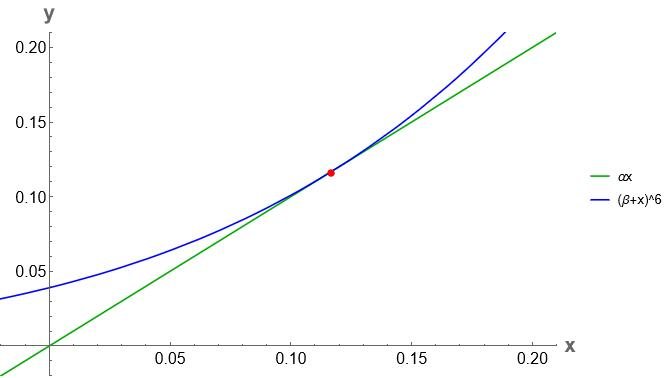
\includegraphics[width=\textwidth]{images/one_intersection.jpg}
            \caption{Одна точка пересечения}
        \end{figure}

        \begin{figure}[ht]
            \centering
            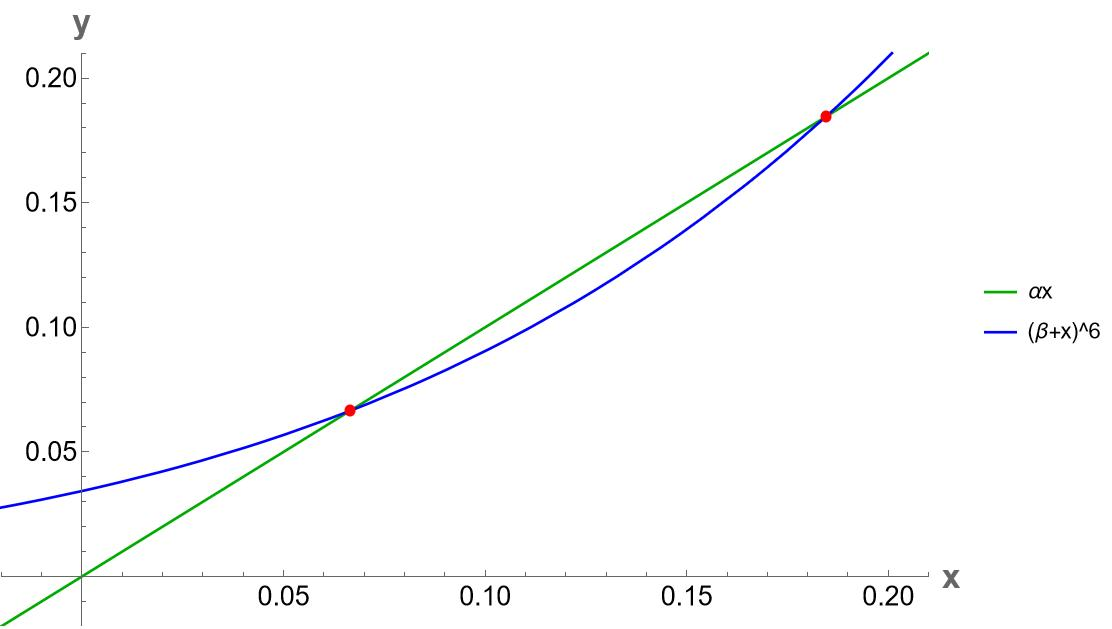
\includegraphics[width=\textwidth]{images/two_intersection.jpg}
            \caption{Две точки пересечения}
        \end{figure}

        \begin{figure}[ht]
            \centering
            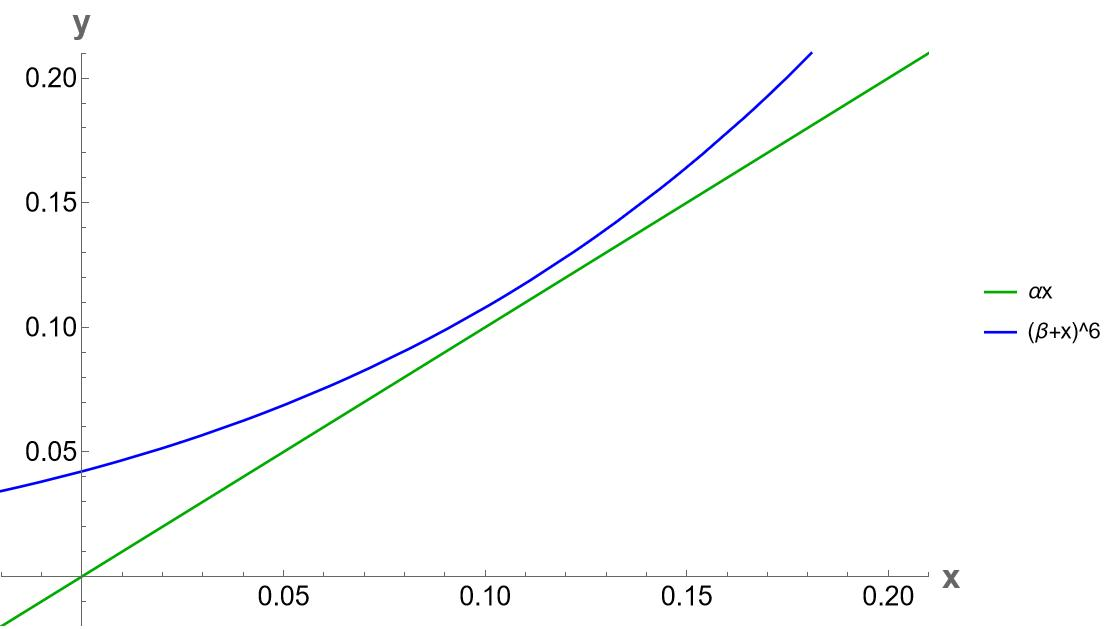
\includegraphics[width=\textwidth]{images/zero_intersection.jpg}
            \caption{Нет точек пересечения}
        \end{figure}

        \begin{figure}[ht]
            \centering
            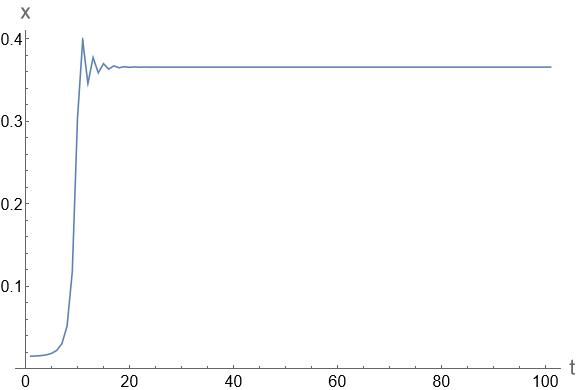
\includegraphics[width=\textwidth]{images/time_series.jpg}
            \caption{Временной ряд}
        \end{figure}

        \begin{figure}[ht]
            \centering
            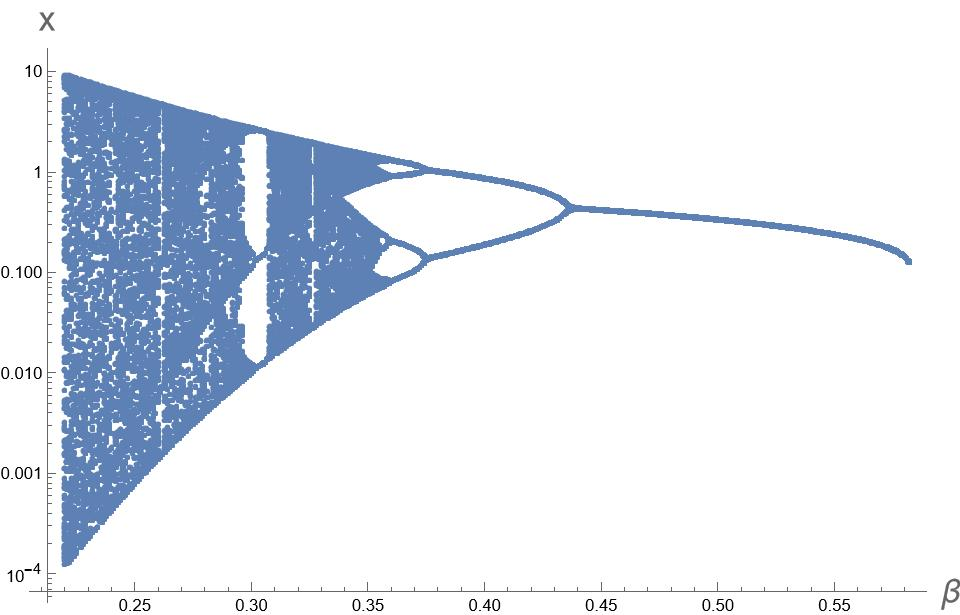
\includegraphics[width=\textwidth]{images/bifurcation.jpg}
            \caption{График бифуркации}
        \end{figure}

\end{document}